\documentclass{beamer}
\usepackage[T1]{fontenc}        % cleaner font
\usepackage[utf8]{inputenc}     % UTF-8 support
\usepackage{xcolor}
\usepackage{color, colortbl}
\usepackage{amsfonts}
\usepackage{subcaption}         % subfigure support
\usepackage{amsmath}
\usepackage[
abbreviate=false,
backend=biber,
sortcites=true,
sorting=nyt,
sortlocale=en_US,
style=numeric,
firstinits=true,
maxnames=10
]{biblatex}
\usepackage{algorithm}
\usepackage{algpseudocode}      % Allow pseudocode
\usepackage{wrapfig}
\usepackage{listings}
\usepackage{color,soul}
\usepackage{tikz}
\usepackage{cancel}

\usetheme{Boadilla}

\newcommand{\setof}[1]{\ensuremath{\left \{ #1 \right \}}}
\newcommand{\tuple}[1]{\ensuremath{\left \langle #1 \right \rangle }}


\title{Contextual Bandit Approach to Targeted Advertising}
\author{Eric Andrews}
\institute{Seminar: Reinforcement Learning and Its Applications\\Department of Computer Science, University of Helsinki}
\date{\today}

\begin{document}

\begin{frame}[plain]
  \titlepage
\end{frame}

\section{Problem description}
\frame{\sectionpage}

\begin{frame}{Online content producers}
  \begin{itemize}
    \item{E.g. News sites, game/movie/music -related sites, search engines etc.}
    \item{Rely on advertisement revenues}
    \item{Banner ads that link to advertisers' sites}
  \end{itemize}
\end{frame}

\begin{frame}{Example of banner advertisement}
  \begin{figure}
    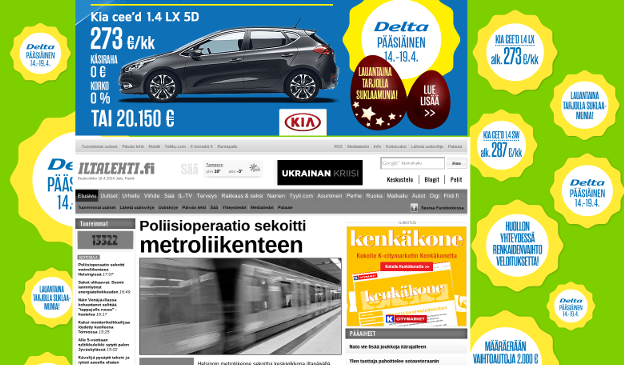
\includegraphics[width=\linewidth]{il.png}
  \end{figure}
\end{frame}

\begin{frame}{Goal}
  \begin{itemize}
    \item{Each click generates some profit.}
    \item{Maximize \emph{click-through rate} (CTR): \#clicks / \#impressions}
    \item{Challenge: can not just fill up page with banners
        \begin{itemize}
          \item{User annoyance}
          \item{Saturation point}
          \item{Lack of room}
        \end{itemize}
      }
    \item{Attempt to intelligently choose ads.}
  \end{itemize}
\end{frame}

\begin{frame}{Targeted and contextual advertising}
  \begin{itemize}
    \item{Model of user: profile, demographics, interests, visited pages etc.}
    \item{\emph{Targeted advertising}: show that banner ad which the user will
      most likely click on.}
    \item[]{}
    \item{Model of content: bag of words, title, author, meta data etc.}
    \item{\emph{Contextual advertising}: show that banner ad which is most
      relevant to the content being served. (Search engines!)}
  \end{itemize}
\end{frame}

\section{Contextual bandit}
\frame{\sectionpage}

\begin{frame}{Targeted advertising as a contextual bandit problem}
  \begin{itemize}
    \item{Assume we have one banner slot.}
    \item{Context $x_t$: profile of user.}
    \item{Actions $a_i \in \mathcal{A}$: the set of ads that can be displayed.}
    \item{Actions $r_t \in \setof{0,1}$: whether the user clicked on the ad.}
    \item{\emph{Learn} relation between context $x_t$ and actions $a_i$ so as
      to maximize reward.}
  \end{itemize}
\end{frame}

\begin{frame}{Targeted advertising as a contextual bandit problem}
  \begin{figure}
    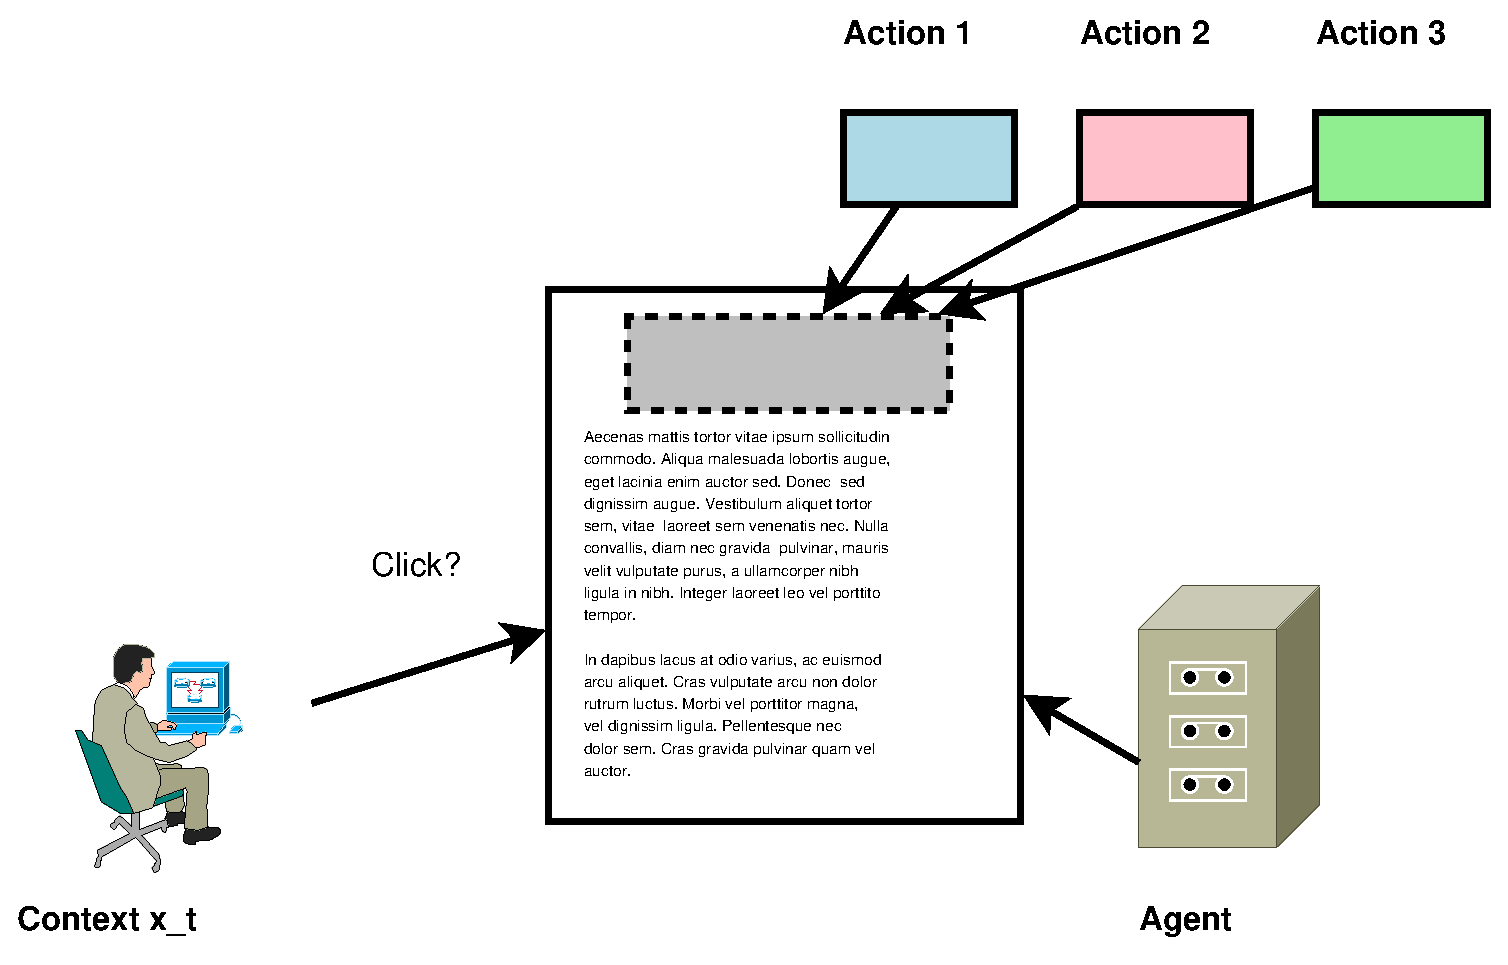
\includegraphics[width=\linewidth]{ta.eps}
  \end{figure}
\end{frame}

\begin{frame}{Contextual bandit setting}
  \begin{itemize}
    \item[]
      \textbf{For} $t = 1, ..., T$ (rounds)
      \begin{enumerate}
        \item{Receive some context $x_t$.}
        \item{Choose action  $a \in \mathcal{A}$ (pull lever).}
        \item{Receive reward $r_t \in \mathbb{R}$.}
      \end{enumerate}
    \item{Given context $x_t$ which lever $a \in \mathcal{A}$ to pull?}
  \end{itemize}
\end{frame}

\section{Thompson sampling}
\frame{\sectionpage}

\begin{frame}{Thompson sampling}
  \begin{itemize}
    \item{Bayesian algorithm to address exploitation vs. exploration}
    \item{Idea: each action-context-pair (ad, user profile) has a probability
      distribution reflecting our belief of its reward payoff.}
    \item{Given context, sample action distributions, pull the action
      corresponding to the largest sample.}
    \item{Update action-context distribution according to whether user clicked
      or not.}
  \end{itemize}
\end{frame}

\begin{frame}{Example case}
  \begin{itemize}
    \item{Assume for simplicity that
        \begin{itemize}
          \item{One banner slot}
          \item{We have contexts (profiles): \textcolor{blue}{republican} or
            \textcolor{red}{democrat}}
          \item{Reward of each ad (action) $R_i \sim
            \mathrm{Bernoulli}(\theta_i^*)$}
        \end{itemize}
      }
    \item{We model our belief of each ad's success probability as
      $$
        \theta_i^* \sim \mathrm{Beta}(1 + S_i, 1 + F_i),
      $$where $S_i$ is \#successes and $F_i$ is \#failures. (conjugate prior)}
  \end{itemize}
\end{frame}

\begin{frame}{Example case}
  \begin{itemize}
    \item{Assume we have three ads that we could show.}
  \end{itemize}
  \begin{figure}
    \centering
    \begin{subfigure}[b]{0.2\textwidth}
      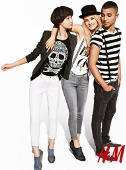
\includegraphics[width=\textwidth]{ad1.png}
      \caption*{Action $a_1$}
    \end{subfigure}
    \begin{subfigure}[b]{0.2\textwidth}
      
\includegraphics[width=\textwidth]{ad2.png}
      \caption*{Action $a_2$}
    \end{subfigure}
    \begin{subfigure}[b]{0.2\textwidth}
      
\includegraphics[width=\textwidth]{ad3.png}
      \caption*{Action $a_3$}
    \end{subfigure}
  \end{figure}
\end{frame}

\begin{frame}
  \begin{figure}
    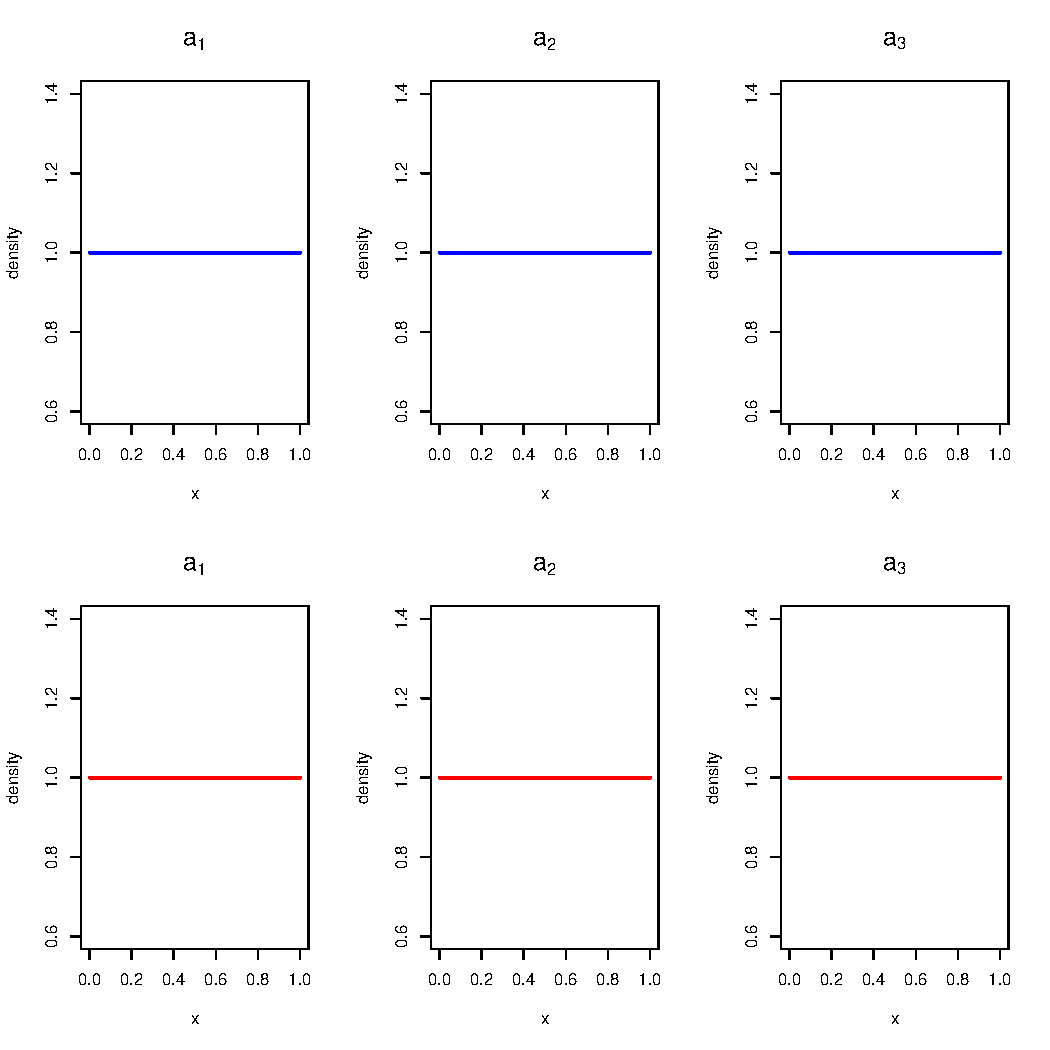
\includegraphics[scale=.4]{b1.pdf}
    \caption{Note: Other priors can be set as well!}
  \end{figure}
\end{frame}

\begin{frame}
  \begin{itemize}
    \item{A user visits the site, context is \textcolor{blue}{republican}}
    \item{Sample three upper distributions, we get: 0.2, 0.4, 0.8}
    \item{Thus action $a_3$ (hamburger ad) is shown to user}
    \item{User does \emph{not} click ad.}
  \end{itemize}
\end{frame}

\begin{frame}
  \begin{figure}
    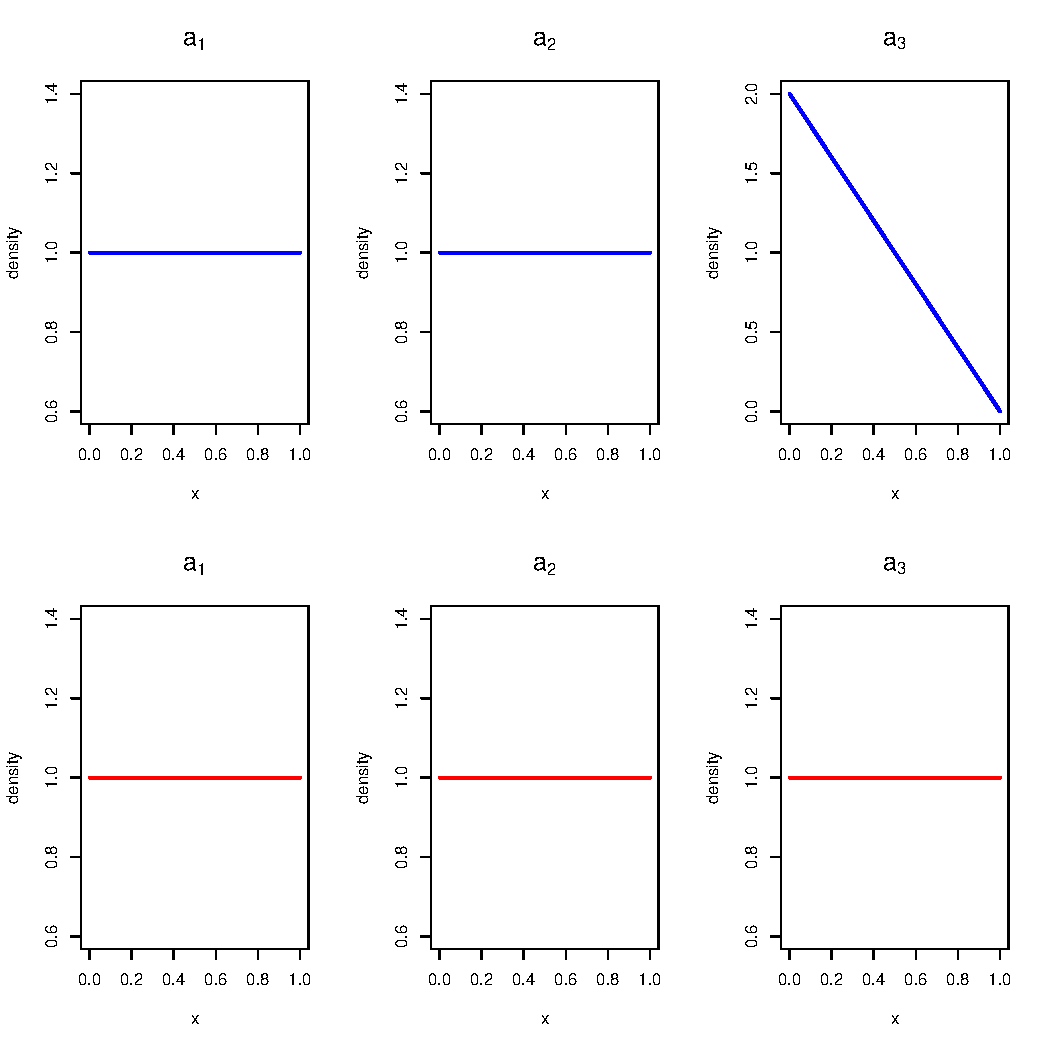
\includegraphics[scale=.5]{b2.pdf}
    \caption{Note: Other priors can be set as well!}
  \end{figure}
\end{frame}

\begin{frame}
  \begin{itemize}
    \item{A user visits the site, context is \textcolor{red}{democrat}}
    \item{Sample three upper distributions, we get: 0.4, 0.9, 0.5}
    \item{Thus action $a_2$ (hamburger ad) is shown to user}
    \item{User does click ad.}
  \end{itemize}
\end{frame}

\begin{frame}
  \begin{figure}
    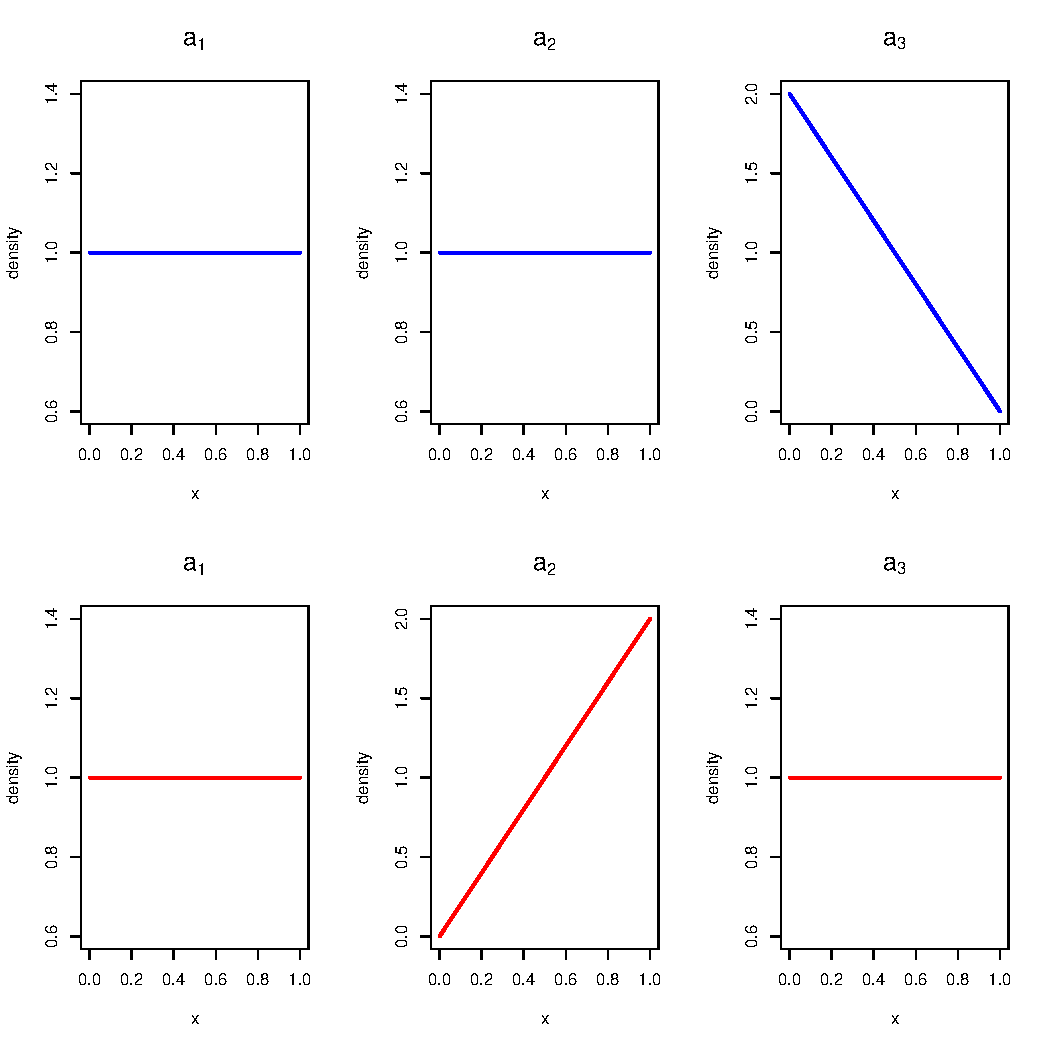
\includegraphics[scale=.5]{b3.pdf}
    \caption{Note: Other priors can be set as well!}
  \end{figure}
\end{frame}

\begin{frame}
  \begin{itemize}
    \item{\textcolor{red}{democract}, $a_2$,  clicks.}
    \item{\textcolor{red}{democract}, $a_2$,  clicks.}
    \item{\textcolor{red}{democract}, $a_2$,  does not click.}
  \end{itemize}
\end{frame}

\begin{frame}
  \begin{figure}
    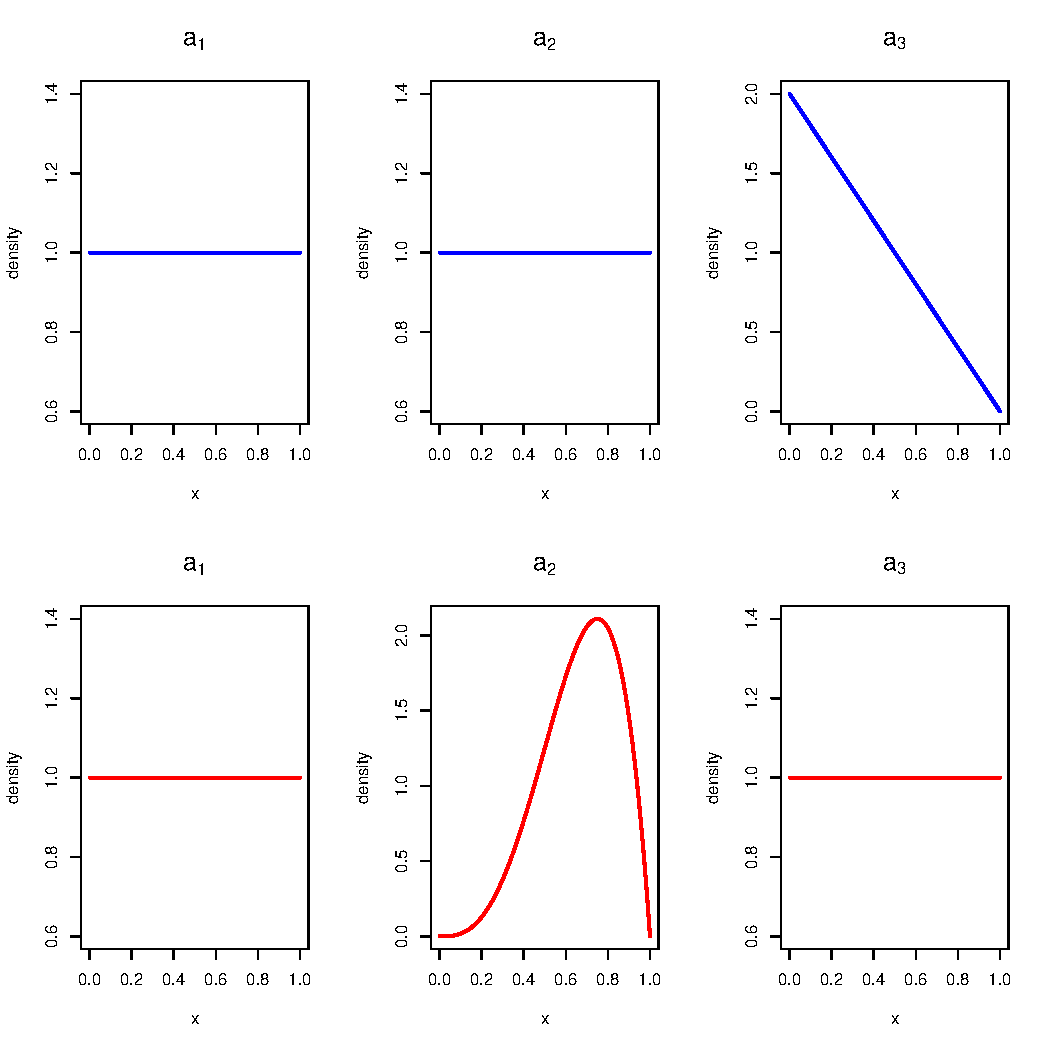
\includegraphics[scale=.5]{b4.pdf}
  \end{figure}
\end{frame}

\begin{frame}
  \begin{itemize}
    \item{\textcolor{blue}{republican}, $a_1$,  clicks.}
    \item{\textcolor{blue}{republican}, $a_3$,  does not click.}
    \item{\textcolor{blue}{republican}, $a_1$,  does not click.}
  \end{itemize}
\end{frame}

\begin{frame}
  \begin{figure}
    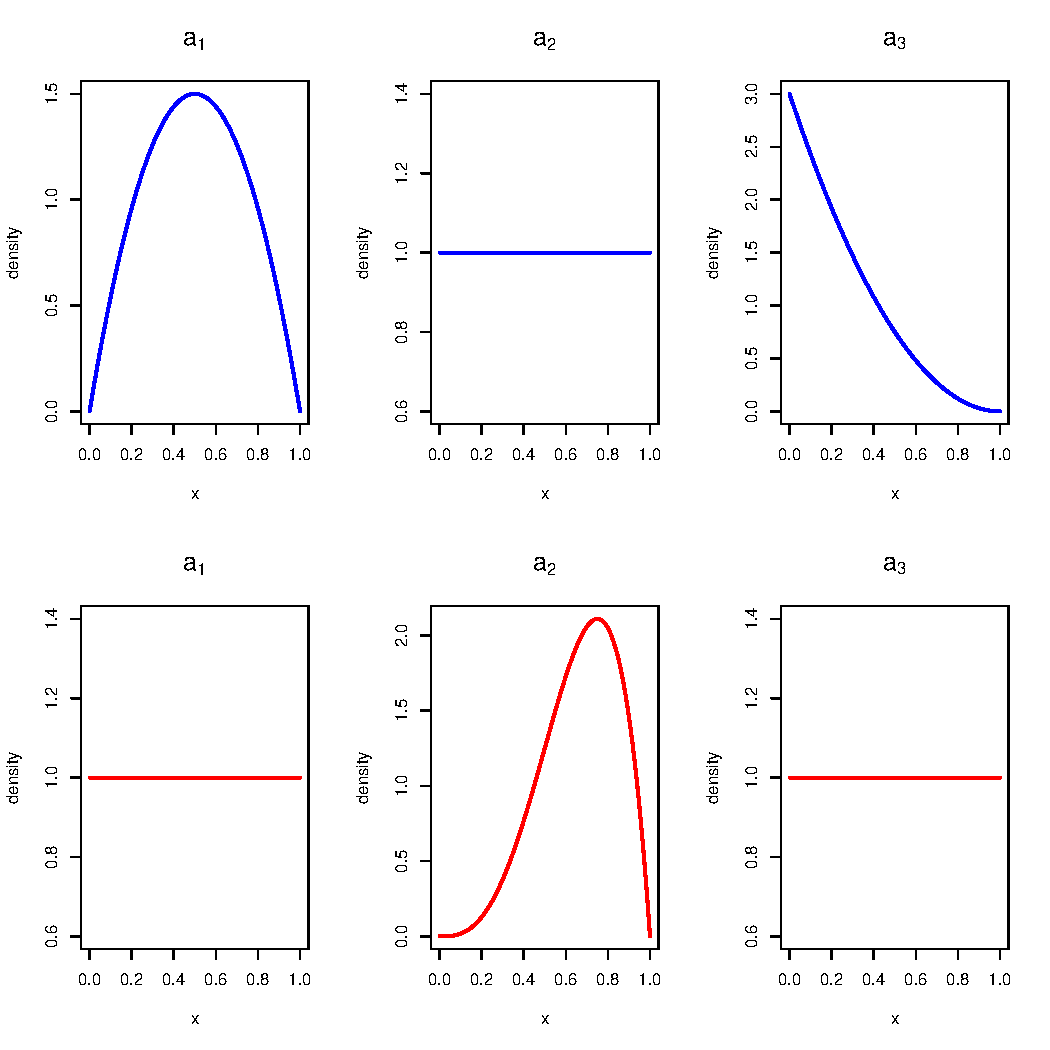
\includegraphics[scale=.5]{b5.pdf}
  \end{figure}
\end{frame}

\begin{frame}{After a while...}
  \begin{figure}
    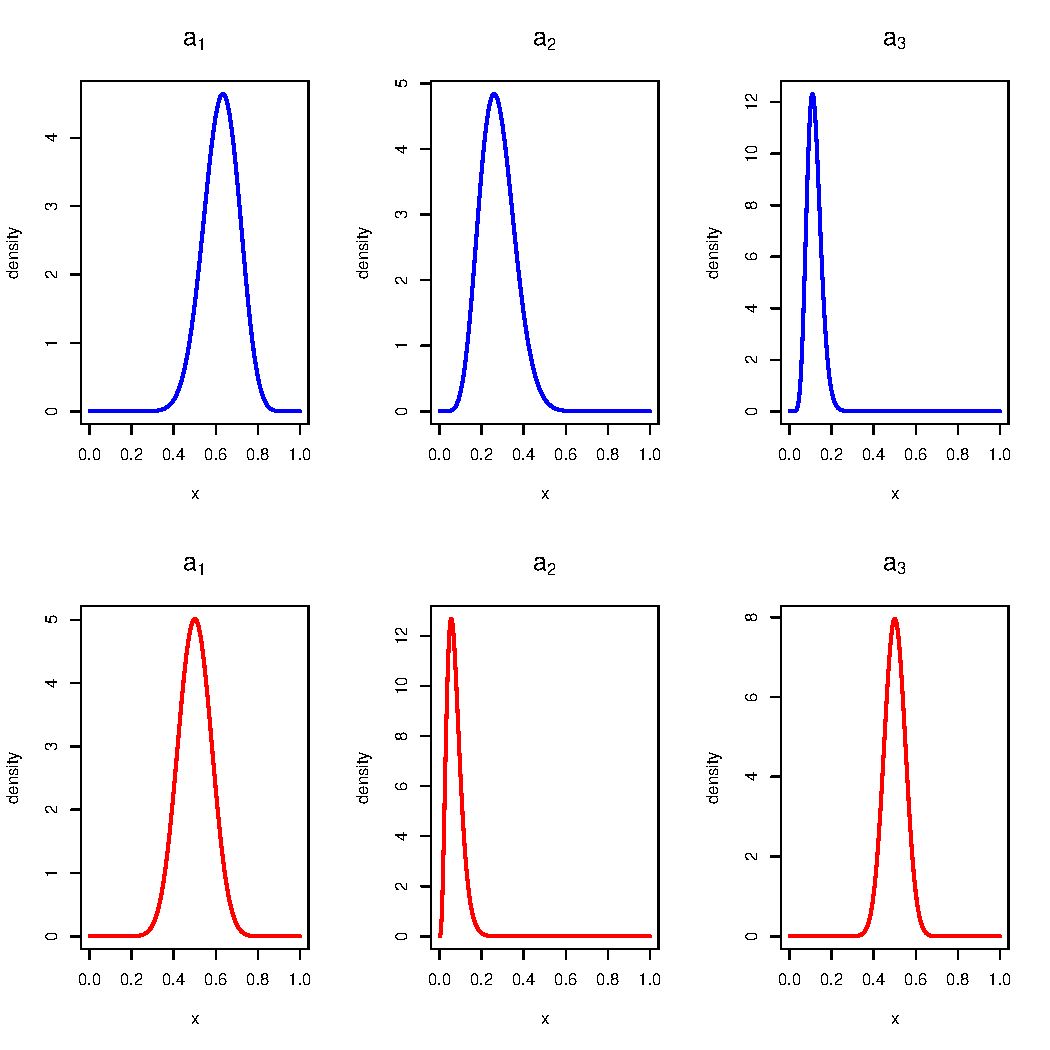
\includegraphics[scale=.45]{b6.pdf}
  \end{figure}
\end{frame}

\begin{frame}{Some points}
  \begin{itemize}
    \item{Keeps exploration open}
    \item{... but starts to exploit when enough experienced gained.}
  \end{itemize}
\end{frame}

\begin{frame}{Pseudocode}
  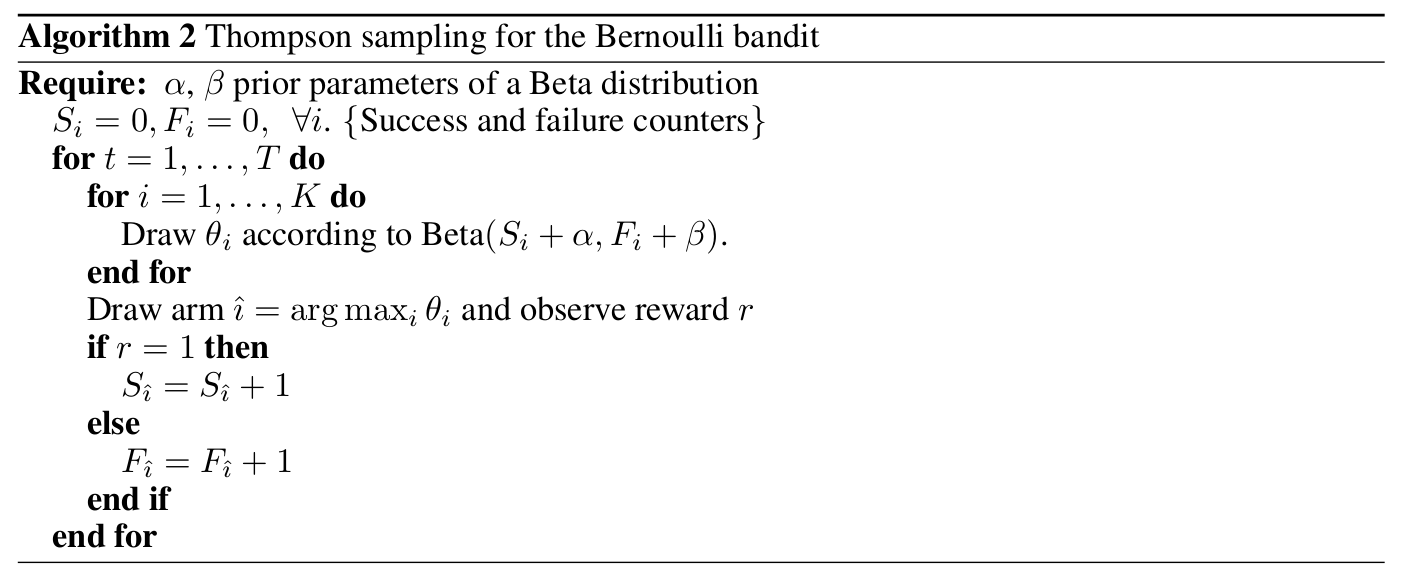
\includegraphics[width=\linewidth]{algo.png}
\end{frame}

\begin{frame}{Compared to UCB}
  \begin{itemize}
    \item[+]{Control amount of exploration vs. exploitation by changing prior
      distributions.}
    \item[+]{Thompson sampling alleviates influence of delayed feedback by
      randomizing over actions vs. UCB deterministiclly chooses}
    \item[-]{Lack of solid theoretical analysis.}
  \end{itemize}
\end{frame}

\section{Mortal bandits}
\frame{\sectionpage}

\begin{frame}{Mortal bandits}
  \begin{itemize}
    \item{Advertisement campaigns have limited lifespans}
    \item{... and new ones spring up.}
    \item{Problem: multi-armed bandit model assumes immortal levers.}
    \item{$\implies$ ample exploration pays off}
  \end{itemize}
\end{frame}

\begin{frame}{Mortal bandits}
  \begin{itemize}
    \item{Optimal regret bound, instead of $O(\ln t)$, we have $\Omega(t)$}
    \item{Especially challenging: many levers, short lifespans}
    \item{Subset heuristic: group subsequent rounds into epochs.}
    \item{At each epoch, randomly choose subset of arms to optimize in.}
    \item{$\implies$ attempt to achieve at least suboptimality.}
  \end{itemize}
\end{frame}

\section{Function approximation}
\frame{\sectionpage}

\begin{frame}{Function approximation}
  \begin{itemize}
    \item{Real world advertisement data sets huge.}
    \item{Lots of information about user.}
    \item{However we need $|\mathcal{A}|$ probabiliy distributions for each
        different context.}
      \item{Use supervised methods, e.g. multivariate linear regression to
        narrow the number of different contexts.}
  \end{itemize}
\end{frame}

\section{Reinforcement learning approaches}
\frame{\sectionpage}

\begin{frame}{RL model more flexible}
  \begin{itemize}
    \item{Capture how user's state (e.g. mood) changes}
    \item{E.g. user attrition caused by an offensive ad.}
    \item{Concurrent interaction between customer and company}
    \item{Delayed rewards}
  \end{itemize}
\end{frame}

\section{Conclusion}
\frame{\sectionpage}

\begin{frame}{Conclusion}
  \begin{itemize}
    \item{Targeted advertising can be approached from a contextual, Bayesian
      multi-armed bandit model.}
    \item{Applying CS to advertising: \emph{computational advertising}.}
    \item{Applied research by Microsoft and Yahoo.}
    \item{Research does not fully disclose many details of real-world systems!}
  \end{itemize}
\end{frame}

\end{document}
